\documentclass{beamer}
\usepackage{amsmath, amssymb, amsthm}
\usepackage{graphicx, fancyhdr}
\usepackage{mdframed} % Add this to the preamble
\usepackage{xcolor} % Ensure xcolor is included
\usepackage{algorithm}
\usepackage{algpseudocode}

\definecolor{Teal}{HTML}{23373B} % Define the color
\definecolor{darkGreen}{rgb}{0.0, 0.5, 0.0}  % Define dark green color
\definecolor{darkBlue}{rgb}{0.0, 0.0, 0.8}  % Define dark green color
\definecolor{gray}{rgb}{0.7, 0.7, 0.7}  % Define dark green color

% Theme choice
\usetheme{metropolis} % Modern and clean layout
% Custom Block Colors
\usepackage{xcolor}
\setbeamercolor{block title}{fg=white, bg=Teal!90} % Block title color
\setbeamercolor{block body}{fg=black, bg=Teal!8}  % Block body color

\newtheorem{conjecture}{Conjecture}
\renewcommand{\thealgorithm}{}
% Footer settings
\setbeamertemplate{footline}{
  \leavevmode\hbox{\begin{beamercolorbox}[wd=\paperwidth,ht=3ex,dp=2ex]{author in head/foot}%
      \hspace{1em} {M. J. Moghaddas Mehr}
      \, \textbar \,
      \insertshorttitle \,
      \textbullet \, 
      \insertsection \, 
      \hfill \insertframenumber{}/\inserttotalframenumber{} \hspace{.5em}
  \end{beamercolorbox}
  }
}

% Title Page Details
\title{Isomorphism in Union-Closed Sets}
\author{Mohammad Javad Moghaddas Mehr}
\institute{Bowling Green State University}
\date{Cincinnati – March 2025}

\begin{document}

% Title Slide
\begin{frame}
	\titlepage
\end{frame}

% Slide 2: History of the Union-Closed Conjecture
\begin{frame}{History}
	In 1979, Péter Frankl proposed a famous conjecture about finite union-closed families.
	He stated that in every such family, there exists an element that appears in at least half of the sets.
	Despite significant efforts, the problem has remained unsolved for more than four decades.
	\vfill
	\pause
	\begin{block}{Union-Closed Conjecture (Frankl, 1979)}
		Let \(\mathcal{K} \subseteq 2^{[n]}\) be a union-closed family of sets.
		Then there exists an element \(i \in \bigcup \mathcal{K}\) such that: \(|\mathcal{K}| \leq 2|\mathcal{K}^i|\),
		where
		\[
			\mathcal{K}^i = \{A \in \mathcal{K} \mid i \in A\}.
		\]
	\end{block}

\end{frame}



\begin{frame}{Examples of Union-Closed Families}
	\textbf{Example 1: Small Family}
	\[
		\mathcal{K} = \{\varnothing, \{1\}, \{1,2\}, \{2,3,4\}, \{1,2,3,4\}\}
	\]
	Here, elements \textbf{1} and \textbf{2} satisfy the conjecture.

	\vfill
	\pause

	\textbf{Example 2: Another Small Family}
	\[
		\mathcal{K} = \{\varnothing, \{a\}, \{b\}, \{a,b\}\}
	\]
	In this case, both \textbf{a} and \textbf{b} satisfy the conjecture.
\end{frame}


\begin{frame}{Isomorphism}
	\begin{itemize}
		\item[\textcolor{orange}{\textbf{?}}]Suppose we have two isomorphic union-closed families. Do the elements have the same frequency counts in both families?
	\end{itemize}

	\vfill
	\pause
	\begin{Definition}
		Let \( \mathcal{K}_1 \) and \( \mathcal{K}_2 \) be union-closed families of sets.
		A bijective mapping \( h: \mathcal{K}_1 \to \mathcal{K}_2 \) is called a \textbf{Isomorphism} if, for all
		\( A_1, A_2 \in \mathcal{K}_1 \), the following property holds:
		\[
			h(A_1 \cup A_2) = h(A_1) \cup h(A_2).
		\]
	\end{Definition}
\end{frame}

\begin{frame}
	\begin{itemize}
		\item[\textcolor{red}{\textbf{X}}] In an isomorphic union-closed family, does each element appear in the same number of sets?
	\end{itemize}
	\pause
	\vfill
	\begin{center}
		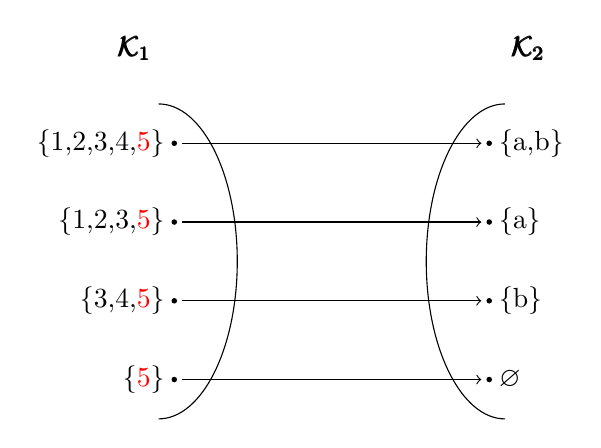
\begin{tikzpicture}[scale=1]
			\draw[thin] (3.2,2) arc[start angle=90, end angle=270, x radius=1, y radius=2]; % X on the right
			\draw[thin] (-1.2,-2) arc[start angle=-90, end angle=90, x radius=1, y radius=2]; % Y on the left
			% Labels for sets
			\node at (-1.5,2.7) {\(\pmb{\mathcal{K}_1}\)};
			\node at (3.5,2.7) {\(\pmb{\mathcal{K}_2}\)};

			% Elements in X (now enclosed in sets)
			\node[left] at (-1,1.5) {\{1,2,3,4,\textcolor{red}{5}\}};
			\node[left] at (-1,0.5) {\{1,2,3,\textcolor{red}{5}\}};
			\node[left] at (-1,-0.5) {\{3,4,\textcolor{red}{5}\}};
			\node[left] at (-1,-1.5) {\{\textcolor{red}{5}\}};

			% Elements in Y (now enclosed in sets)
			\node[right] at (3,1.5) {\{a,b\}};
			\node[right] at (3,0.5) {\{a\}};
			\node[right] at (3,-0.5) {\{b\}};
			\node[right] at (3,-1.5) {\(\varnothing\)};


			% Draw mappings
			\draw[->, thin] (-.9,1.5) -- (2.9,1.5);
			\draw[->, thin] (-.9,0.5) -- (2.9,0.5);
			\draw[->, thin] (-.9,-0.5) -- (2.9,-0.5);
			\draw[->, thin] (-.9,-1.5) -- (2.9,-1.5);

			% Draw points in X
			\foreach \y in {1.5,0.5,-0.5,-1.5}
			\fill (-1,\y) circle (1pt);

			% Draw points in Y
			\foreach \y in {1.5,0.5,-0.5,-1.5}
			\fill (3,\y) circle (1pt);
		\end{tikzpicture}
	\end{center}

\end{frame}

\begin{frame}

	\begin{itemize}
		\item[\textcolor{red}{\textbf{X}}] In an isomorphic union-closed family, does each element appear in the same number of sets?
	\end{itemize}

	\vfill
	\begin{center}
		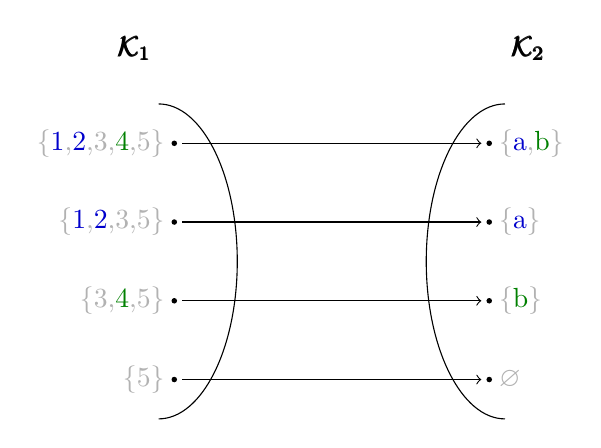
\begin{tikzpicture}[scale=1]
			\draw[thin] (3.2,2) arc[start angle=90, end angle=270, x radius=1, y radius=2]; % X on the right
			\draw[thin] (-1.2,-2) arc[start angle=-90, end angle=90, x radius=1, y radius=2]; % Y on the left
			% Labels for sets
			\node at (-1.5,2.7) {\(\pmb{\mathcal{K}_1}\)};
			\node at (3.5,2.7) {\(\pmb{\mathcal{K}_2}\)};

			% Elements in X (now enclosed in sets)

			\node[left] at (-1,1.5) {\textcolor{gray}{\{\textcolor{darkBlue}{1},\textcolor{darkBlue}{2},3,\textcolor{darkGreen}{4},5\}}};
			\node[left] at (-1,0.5) {\textcolor{gray}{\{\textcolor{darkBlue}{1},\textcolor{darkBlue}{2},3,5\}}};
			\node[left] at (-1,-0.5) {\textcolor{gray}{\{3,\textcolor{darkGreen}{4},5\}}};
			\node[left] at (-1,-1.5) {\textcolor{gray}{\{5\}}};


			% Elements in Y (now enclosed in sets)
			\node[right] at (3,1.5) {\textcolor{gray}{\{\textcolor{darkBlue}{a},\textcolor{darkGreen}{b}\}}};
			\node[right] at (3,0.5) {\textcolor{gray}{\{\textcolor{darkBlue}{a}\}}};
			\node[right] at (3,-0.5) {\textcolor{gray}{\{\textcolor{darkGreen}{b}\}}};
			\node[right] at (3,-1.5) {\textcolor{gray}{\(\varnothing\)}};



			% Draw mappings
			\draw[->, thin] (-.9,1.5) -- (2.9,1.5);
			\draw[->, thin] (-.9,0.5) -- (2.9,0.5);
			\draw[->, thin] (-.9,-0.5) -- (2.9,-0.5);
			\draw[->, thin] (-.9,-1.5) -- (2.9,-1.5);

			% Draw points in X
			\foreach \y in {1.5,0.5,-0.5,-1.5}
			\fill (-1,\y) circle (1pt);

			% Draw points in Y
			\foreach \y in {1.5,0.5,-0.5,-1.5}
			\fill (3,\y) circle (1pt);
		\end{tikzpicture}
	\end{center}
\end{frame}


\begin{frame}
	\centering
	\begin{minipage}{0.4\textwidth}
		\centering
		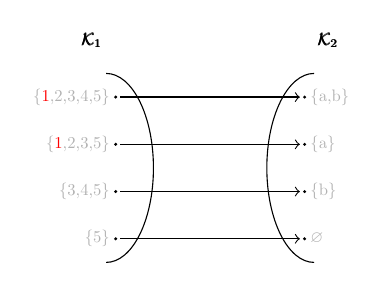
\begin{tikzpicture}[scale=0.6, transform shape]
			\draw[thin] (3.2,2) arc[start angle=90, end angle=270, x radius=1, y radius=2]; % X on the right
			\draw[thin] (-1.2,-2) arc[start angle=-90, end angle=90, x radius=1, y radius=2]; % Y on the left
			% Labels for sets
			\node at (-1.5,2.7) {\(\pmb{\mathcal{K}_1}\)};
			\node at (3.5,2.7) {\(\pmb{\mathcal{K}_2}\)};

			% Elements in X (now enclosed in sets)
			\node[left] at (-1,1.5) {\textcolor{gray}{\{\textcolor{red}1,2,3,4,5\}}};
			\node[left] at (-1,0.5) {\textcolor{gray}{\{\textcolor{red}1,2,3,5\}}};
			\node[left] at (-1,-0.5) {\textcolor{gray}{\{3,4,5\}}};
			\node[left] at (-1,-1.5) {\textcolor{gray}{\{5\}}};

			% Elements in Y (now enclosed in sets)
			\node[right] at (3,1.5) {\textcolor{gray}{\{a,b\}}};
			\node[right] at (3,0.5) {\textcolor{gray}{\{a\}}};
			\node[right] at (3,-0.5) {\textcolor{gray}{\{b\}}};
			\node[right] at (3,-1.5) {\textcolor{gray}{\(\varnothing\)}};

			% Draw mappings
			\draw[->, thin] (-.9,1.5) -- (2.9,1.5);
			\draw[->, thin] (-.9,0.5) -- (2.9,0.5);
			\draw[->, thin] (-.9,-0.5) -- (2.9,-0.5);
			\draw[->, thin] (-.9,-1.5) -- (2.9,-1.5);

			% Draw points in X
			\foreach \y in {1.5,0.5,-0.5,-1.5}
			\fill (-1,\y) circle (1pt);

			% Draw points in Y
			\foreach \y in {1.5,0.5,-0.5,-1.5}
			\fill (3,\y) circle (1pt);
		\end{tikzpicture}
	\end{minipage}
	\hspace{.5cm}
	% Second diagram
	\begin{minipage}{0.4\textwidth}
		\centering
		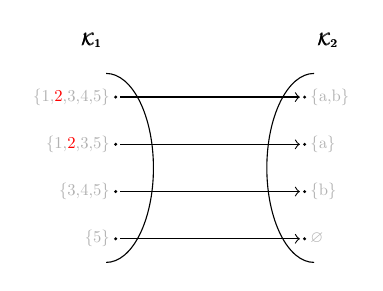
\begin{tikzpicture}[scale=0.6, transform shape]
			\draw[thin] (3.2,2) arc[start angle=90, end angle=270, x radius=1, y radius=2]; % X on the right
			\draw[thin] (-1.2,-2) arc[start angle=-90, end angle=90, x radius=1, y radius=2]; % Y on the left
			% Labels for sets
			\node at (-1.5,2.7) {\(\pmb{\mathcal{K}_1}\)};
			\node at (3.5,2.7) {\(\pmb{\mathcal{K}_2}\)};

			% Elements in X (now enclosed in sets)
			\node[left] at (-1,1.5) {\textcolor{gray}{\{1,\textcolor{red}2,3,4,5\}}};
			\node[left] at (-1,0.5) {\textcolor{gray}{\{1,\textcolor{red}2,3,5\}}};
			\node[left] at (-1,-0.5) {\textcolor{gray}{\{3,4,5\}}};
			\node[left] at (-1,-1.5) {\textcolor{gray}{\{5\}}};

			% Elements in Y (now enclosed in sets)
			\node[right] at (3,1.5) {\textcolor{gray}{\{a,b\}}};
			\node[right] at (3,0.5) {\textcolor{gray}{\{a\}}};
			\node[right] at (3,-0.5) {\textcolor{gray}{\{b\}}};
			\node[right] at (3,-1.5) {\textcolor{gray}{\(\varnothing\)}};

			% Draw mappings
			\draw[->, thin] (-.9,1.5) -- (2.9,1.5);
			\draw[->, thin] (-.9,0.5) -- (2.9,0.5);
			\draw[->, thin] (-.9,-0.5) -- (2.9,-0.5);
			\draw[->, thin] (-.9,-1.5) -- (2.9,-1.5);

			% Draw points in X
			\foreach \y in {1.5,0.5,-0.5,-1.5}
			\fill (-1,\y) circle (1pt);

			% Draw points in Y
			\foreach \y in {1.5,0.5,-0.5,-1.5}
			\fill (3,\y) circle (1pt);
		\end{tikzpicture}
	\end{minipage}
	\vfill
	\pause
	\begin{minipage}{0.4\textwidth}
		\centering
		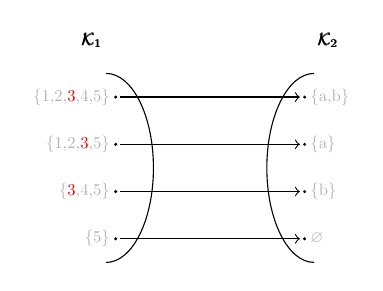
\begin{tikzpicture}[scale=0.6, transform shape]
			\draw[thin] (3.2,2) arc[start angle=90, end angle=270, x radius=1, y radius=2]; % X on the right
			\draw[thin] (-1.2,-2) arc[start angle=-90, end angle=90, x radius=1, y radius=2]; % Y on the left
			% Labels for sets
			\node at (-1.5,2.7) {\(\pmb{\mathcal{K}_1}\)};
			\node at (3.5,2.7) {\(\pmb{\mathcal{K}_2}\)};

			% Elements in X (now enclosed in sets)
			\node[left] at (-1,1.5) {\textcolor{gray}{\{1,2,\textcolor{red}3,4,5\}}};
			\node[left] at (-1,0.5) {\textcolor{gray}{\{1,2,\textcolor{red}3,5\}}};
			\node[left] at (-1,-0.5) {\textcolor{gray}{\{\textcolor{red}3,4,5\}}};
			\node[left] at (-1,-1.5) {\textcolor{gray}{\{5\}}};

			% Elements in Y (now enclosed in sets)
			\node[right] at (3,1.5) {\textcolor{gray}{\{a,b\}}};
			\node[right] at (3,0.5) {\textcolor{gray}{\{a\}}};
			\node[right] at (3,-0.5) {\textcolor{gray}{\{b\}}};
			\node[right] at (3,-1.5) {\textcolor{gray}{\(\varnothing\)}};

			% Draw mappings
			\draw[->, thin] (-.9,1.5) -- (2.9,1.5);
			\draw[->, thin] (-.9,0.5) -- (2.9,0.5);
			\draw[->, thin] (-.9,-0.5) -- (2.9,-0.5);
			\draw[->, thin] (-.9,-1.5) -- (2.9,-1.5);

			% Draw points in X
			\foreach \y in {1.5,0.5,-0.5,-1.5}
			\fill (-1,\y) circle (1pt);

			% Draw points in Y
			\foreach \y in {1.5,0.5,-0.5,-1.5}
			\fill (3,\y) circle (1pt);
		\end{tikzpicture}
	\end{minipage}
	\hspace{.5cm}
	% Second diagram
	\begin{minipage}{0.4\textwidth}
		\centering
		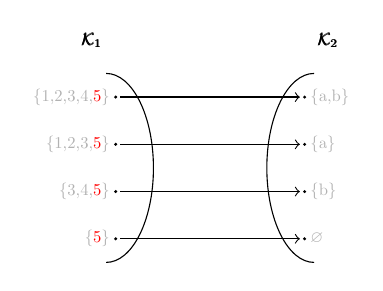
\begin{tikzpicture}[scale=0.6, transform shape]
			\draw[thin] (3.2,2) arc[start angle=90, end angle=270, x radius=1, y radius=2]; % X on the right
			\draw[thin] (-1.2,-2) arc[start angle=-90, end angle=90, x radius=1, y radius=2]; % Y on the left
			% Labels for sets
			\node at (-1.5,2.7) {\(\pmb{\mathcal{K}_1}\)};
			\node at (3.5,2.7) {\(\pmb{\mathcal{K}_2}\)};

			% Elements in X (now enclosed in sets)
			\node[left] at (-1,1.5) {\textcolor{gray}{\{1,2,3,4,\textcolor{red}5\}}};
			\node[left] at (-1,0.5) {\textcolor{gray}{\{1,2,3,\textcolor{red}5\}}};
			\node[left] at (-1,-0.5) {\textcolor{gray}{\{3,4,\textcolor{red}5\}}};
			\node[left] at (-1,-1.5) {\textcolor{gray}{\{\textcolor{red}5\}}};

			% Elements in Y (now enclosed in sets)
			\node[right] at (3,1.5) {\textcolor{gray}{\{a,b\}}};
			\node[right] at (3,0.5) {\textcolor{gray}{\{a\}}};
			\node[right] at (3,-0.5) {\textcolor{gray}{\{b\}}};
			\node[right] at (3,-1.5) {\textcolor{gray}{\(\varnothing\)}};

			% Draw mappings
			\draw[->, thin] (-.9,1.5) -- (2.9,1.5);
			\draw[->, thin] (-.9,0.5) -- (2.9,0.5);
			\draw[->, thin] (-.9,-0.5) -- (2.9,-0.5);
			\draw[->, thin] (-.9,-1.5) -- (2.9,-1.5);

			% Draw points in X
			\foreach \y in {1.5,0.5,-0.5,-1.5}
			\fill (-1,\y) circle (1pt);

			% Draw points in Y
			\foreach \y in {1.5,0.5,-0.5,-1.5}
			\fill (3,\y) circle (1pt);
		\end{tikzpicture}
	\end{minipage}

\end{frame}

\begin{frame}
	\begin{definition}
		Let \( \mathcal{K} \subseteq 2^{[n]} \). An element \( z \in \bigcup \mathcal{K} \) is called \textbf{redundant}, if removing \( z \) from every set in \( \mathcal{K} \) does not change the size of the collection. Specifically, we define:
		\[
			\mathcal{K}^{\setminus z} = \{X \setminus \{z\} \mid X \in \mathcal{K}\},
		\]
		where \( |\mathcal{K}| = |\mathcal{K}^{\setminus z}| \). The collection \( \mathcal{K}^{\setminus z} \) is called the \textbf{reduced collection}.
	\end{definition}
	\pause
	\vfill

	\begin{definition}
		A collection \(\mathcal{K} \subseteq 2^{[n]}\) is called \textbf{pure} if it does not have any \textbf{redundant} element.
	\end{definition}
\end{frame}


\begin{frame}
	\centering
	\begin{minipage}{0.4\textwidth}
		\centering
		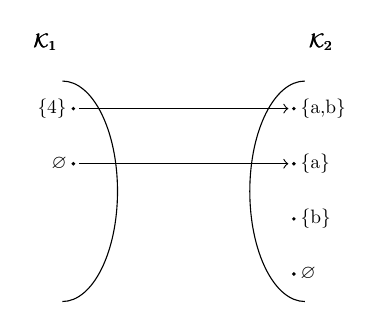
\begin{tikzpicture}[scale=.7, transform shape]
			\draw[thin] (3.2,2) arc[start angle=90, end angle=270, x radius=1, y radius=2]; % X on the right
			\draw[thin] (-1.2,-2) arc[start angle=-90, end angle=90, x radius=1, y radius=2]; % Y on the left
			% Labels for sets
			\node at (-1.5,2.7) {\(\pmb{\mathcal{K}_1}\)};
			\node at (3.5,2.7) {\(\pmb{\mathcal{K}_2}\)};

			% Elements in X (now enclosed in sets)
			\node[left] at (-1,1.5) {\{4\}};
			\node[left] at (-1,0.5) {\(\varnothing\)};

			% Elements in Y (now enclosed in sets)
			\node[right] at (3,1.5) {\{a,b\}};
			\node[right] at (3,0.5) {\{a\}};
			\node[right] at (3,-0.5) {\{b\}};
			\node[right] at (3,-1.5) {\(\varnothing\)};


			% Draw mappings
			\draw[->, thin] (-.9,1.5) -- (2.9,1.5);
			\draw[->, thin] (-.9,0.5) -- (2.9,0.5);

			% Draw points in X
			\foreach \y in {1.5,0.5}
			\fill (-1,\y) circle (1pt);

			% Draw points in Y
			\foreach \y in {1.5,0.5,-0.5,-1.5}
			\fill (3,\y) circle (1pt);
		\end{tikzpicture}
	\end{minipage}
	\hspace{.5cm}
	\vfill
	\pause
	\begin{minipage}{0.4\textwidth}
		\centering
		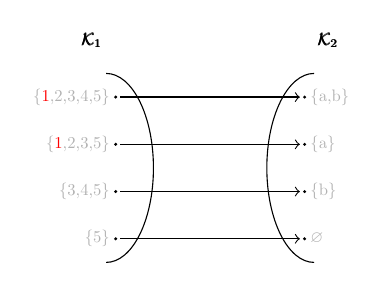
\begin{tikzpicture}[scale=0.6, transform shape]
			\draw[thin] (3.2,2) arc[start angle=90, end angle=270, x radius=1, y radius=2]; % X on the right
			\draw[thin] (-1.2,-2) arc[start angle=-90, end angle=90, x radius=1, y radius=2]; % Y on the left
			% Labels for sets
			\node at (-1.5,2.7) {\(\pmb{\mathcal{K}_1}\)};
			\node at (3.5,2.7) {\(\pmb{\mathcal{K}_2}\)};

			% Elements in X (now enclosed in sets)
			\node[left] at (-1,1.5) {\textcolor{gray}{\{\textcolor{red}1,2,3,4,5\}}};
			\node[left] at (-1,0.5) {\textcolor{gray}{\{\textcolor{red}1,2,3,5\}}};
			\node[left] at (-1,-0.5) {\textcolor{gray}{\{3,4,5\}}};
			\node[left] at (-1,-1.5) {\textcolor{gray}{\{5\}}};

			% Elements in Y (now enclosed in sets)
			\node[right] at (3,1.5) {\textcolor{gray}{\{a,b\}}};
			\node[right] at (3,0.5) {\textcolor{gray}{\{a\}}};
			\node[right] at (3,-0.5) {\textcolor{gray}{\{b\}}};
			\node[right] at (3,-1.5) {\textcolor{gray}{\(\varnothing\)}};

			% Draw mappings
			\draw[->, thin] (-.9,1.5) -- (2.9,1.5);
			\draw[->, thin] (-.9,0.5) -- (2.9,0.5);
			\draw[->, thin] (-.9,-0.5) -- (2.9,-0.5);
			\draw[->, thin] (-.9,-1.5) -- (2.9,-1.5);

			% Draw points in X
			\foreach \y in {1.5,0.5,-0.5,-1.5}
			\fill (-1,\y) circle (1pt);

			% Draw points in Y
			\foreach \y in {1.5,0.5,-0.5,-1.5}
			\fill (3,\y) circle (1pt);
		\end{tikzpicture}
	\end{minipage}
	\hspace{.5cm}
	% Second diagram
	\begin{minipage}{0.4\textwidth}
		\centering
		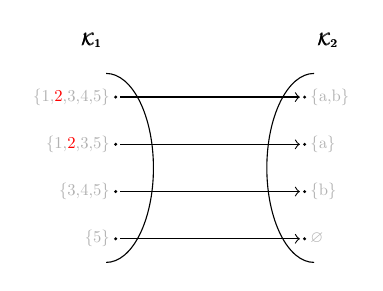
\begin{tikzpicture}[scale=0.6, transform shape]
			\draw[thin] (3.2,2) arc[start angle=90, end angle=270, x radius=1, y radius=2]; % X on the right
			\draw[thin] (-1.2,-2) arc[start angle=-90, end angle=90, x radius=1, y radius=2]; % Y on the left
			% Labels for sets
			\node at (-1.5,2.7) {\(\pmb{\mathcal{K}_1}\)};
			\node at (3.5,2.7) {\(\pmb{\mathcal{K}_2}\)};

			% Elements in X (now enclosed in sets)
			\node[left] at (-1,1.5) {\textcolor{gray}{\{1,\textcolor{red}2,3,4,5\}}};
			\node[left] at (-1,0.5) {\textcolor{gray}{\{1,\textcolor{red}2,3,5\}}};
			\node[left] at (-1,-0.5) {\textcolor{gray}{\{3,4,5\}}};
			\node[left] at (-1,-1.5) {\textcolor{gray}{\{5\}}};

			% Elements in Y (now enclosed in sets)
			\node[right] at (3,1.5) {\textcolor{gray}{\{a,b\}}};
			\node[right] at (3,0.5) {\textcolor{gray}{\{a\}}};
			\node[right] at (3,-0.5) {\textcolor{gray}{\{b\}}};
			\node[right] at (3,-1.5) {\textcolor{gray}{\(\varnothing\)}};

			% Draw mappings
			\draw[->, thin] (-.9,1.5) -- (2.9,1.5);
			\draw[->, thin] (-.9,0.5) -- (2.9,0.5);
			\draw[->, thin] (-.9,-0.5) -- (2.9,-0.5);
			\draw[->, thin] (-.9,-1.5) -- (2.9,-1.5);

			% Draw points in X
			\foreach \y in {1.5,0.5,-0.5,-1.5}
			\fill (-1,\y) circle (1pt);

			% Draw points in Y
			\foreach \y in {1.5,0.5,-0.5,-1.5}
			\fill (3,\y) circle (1pt);
		\end{tikzpicture}
	\end{minipage}
\end{frame}


\begin{frame}{Redundancy Removal Algorithm}
	\begin{algorithm}[H]
		\caption[o]{Redundancy Removal}
		\begin{algorithmic}[1]
			\While{redundant elements exist}
			\State Identify all redundant elements
			\State Remove one redundant element
			\EndWhile
		\end{algorithmic}
	\end{algorithm}
	\vfill
	\pause

	\begin{block}{Purified Collection}
		The \textbf{Purified Collection} of \( \mathcal{K} \), denoted by \( \mathcal{K}^* \), is constructed by iteratively removing all redundant elements from \( \mathcal{K} \).
	\end{block}

\end{frame}


\begin{frame}{Notes on \texorpdfstring{$K^*$}{K*}}
	\begin{itemize}
		\item $K^*$ is not well-defined — there are many ways to purify a family!
		      \begin{itemize}
			      \item Fortunately, all versions of $K^*$ are \textbf{isomorphic}.
			      \item So $K^*$ is unique \textit{up to isomorphism}.
		      \end{itemize}
		      \vspace{0.5em}
		\item The main issue: we don’t know how many steps are needed to reach $K^*$.
		      \begin{itemize}
			      \item Different orders of removing redundant elements may lead to faster purification.
			      \item We might end up with families of different sizes — even though they are isomorphic.
		      \end{itemize}
		      \vspace{0.5em}
		\item That’s not very satisfying to me.
	\end{itemize}
\end{frame}

\begin{frame}

	\begin{itemize}
		\item[\textcolor{darkGreen}{\textbf{\checkmark}}]	If a \textbf{pure union-closed family} satisfies Frankl’s conjecture, does every isomorphic family also satisfy it?
		\item[\textcolor{darkGreen}{\textbf{\checkmark}}] In an isomorphic \textbf{pure union-closed family}, does each element appear in the same number of sets?
	\end{itemize}

	\vfill
	\begin{center}
		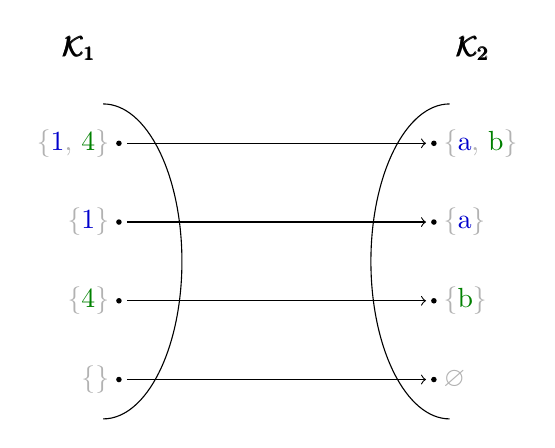
\begin{tikzpicture}[scale=1]
			\draw[thin] (3.2,2) arc[start angle=90, end angle=270, x radius=1, y radius=2]; % X on the right
			\draw[thin] (-1.2,-2) arc[start angle=-90, end angle=90, x radius=1, y radius=2]; % Y on the left
			% Labels for sets
			\node at (-1.5,2.7) {\(\pmb{\mathcal{K}_1}\)};
			\node at (3.5,2.7) {\(\pmb{\mathcal{K}_2}\)};

			% Elements in X (now enclosed in sets)
			\node[left] at (-1,1.5) {\textcolor{gray}{\{\textcolor{darkBlue}{1}, \textcolor{darkGreen}{4}\}}};
			\node[left] at (-1,0.5) {\textcolor{gray}{\{\textcolor{darkBlue}{1}\}}};
			\node[left] at (-1,-0.5) {\textcolor{gray}{\{\textcolor{darkGreen}{4}\}}};
			\node[left] at (-1,-1.5) {\textcolor{gray}{\{\}}};


			% Elements in Y (now enclosed in sets)
			\node[right] at (3,1.5) {\textcolor{gray}{\{\textcolor{darkBlue}{a}, \textcolor{darkGreen}{b}\}}};
			\node[right] at (3,0.5) {\textcolor{gray}{\{\textcolor{darkBlue}{a}\}}};
			\node[right] at (3,-0.5) {\textcolor{gray}{\{\textcolor{darkGreen}{b}\}}};
			\node[right] at (3,-1.5) {\textcolor{gray}{\(\varnothing\)}};



			% Draw mappings
			\draw[->, thin] (-.9,1.5) -- (2.9,1.5);
			\draw[->, thin] (-.9,0.5) -- (2.9,0.5);
			\draw[->, thin] (-.9,-0.5) -- (2.9,-0.5);
			\draw[->, thin] (-.9,-1.5) -- (2.9,-1.5);

			% Draw points in X
			\foreach \y in {1.5,0.5,-0.5,-1.5}
			\fill (-1,\y) circle (1pt);

			% Draw points in Y
			\foreach \y in {1.5,0.5,-0.5,-1.5}
			\fill (3,\y) circle (1pt);
		\end{tikzpicture}
	\end{center}
\end{frame}

\begin{frame}
	\begin{theorem}[Cardinality]
		Let \( \mathcal{K}_1 \) and \( \mathcal{K}_2 \) be \textit{\hyperref[def:pure_collection]{pure union-closed families of sets}}. If there exists an isomorphism \( h: \mathcal{K}_1 \to \mathcal{K}_2 \), then for every \( A \in \mathcal{K}_1 \), we have:
		\[
			|A| = |h(A)|.
		\]
	\end{theorem}
	\pause
	\vfill
	\begin{corollary}[Old Version]
		Let \( \mathcal{K}_1 \) and \( \mathcal{K}_2 \) be \textit{\hyperref[def:pure_collection]{pure union-closed families of sets}}. If there exists an isomorphism \( h: \mathcal{K}_1 \to \mathcal{K}_2 \), we have:
		\[
			\left| \bigcup\mathcal{K}_1 \right| = \left| \bigcup\mathcal{K}_2 \right|.
		\]
	\end{corollary}

\end{frame}

\begin{frame}
	\begin{corollary}
		Let \( \mathcal{K}_1 \) and \( \mathcal{K}_2 \) be pure union-closed families of sets. If there exists an isomorphism \( h: \mathcal{K}_1 \to \mathcal{K}_2 \), then for any \(A, B \in \mathcal{K}_1\), the following properties hold:
		\begin{enumerate}
			\item \(|A \cup B| = |h(A) \cup h(B)|\).
			\item \(|A \cap B| = |h(A) \cap h(B)|\).
			\item \(|A \setminus B| = |h(A) \setminus h(B)|\).
			\item \(|A^c| = |h{(A)}^c|\),
		\end{enumerate}
		where \(A^c = \bigcup \mathcal{K}_1 \setminus A\) and
		\(h{(A)}^c = {\bigcup \mathcal{K}_2} \setminus h(A)\).

	\end{corollary}
\end{frame}

\begin{frame}

	\begin{theorem}
		Let \( \mathcal{K}_1 \) and \( \mathcal{K}_2 \) be pure union-closed families of sets. For every isomorphism \( h: \mathcal{K}_1 \to \mathcal{K}_2 \), there exists a \textbf{hyperisomorphism} \( H: \bigcup \mathcal{K}_1 \to \bigcup \mathcal{K}_2 \) such that:
		\[
			h(A) = \{ H(a) \mid a \in A \} \quad \text{for all } A \in \mathcal{K}_1.
		\]
	\end{theorem}

\end{frame}

\begin{frame}
	\frametitle{References}
	\nocite{*} % Include all references
	\bibliographystyle{plainurl}
	\bibliography{references}
\end{frame}

\begin{frame}{Thank You!}
	\textbf{Any Questions?}
	\begin{itemize}
		\item Email: m.moghadas11235@gmail.com
		\item Paper available on \href{https://arxiv.org/abs/2501.02637v2}{ArXiv}.
	\end{itemize}
\end{frame}





\end{document}
